% Options for packages loaded elsewhere
\PassOptionsToPackage{unicode}{hyperref}
\PassOptionsToPackage{hyphens}{url}
\PassOptionsToPackage{dvipsnames,svgnames,x11names}{xcolor}
%
\documentclass[
  11pt,
]{article}
\usepackage{amsmath,amssymb}
\usepackage{iftex}
\ifPDFTeX
  \usepackage[T1]{fontenc}
  \usepackage[utf8]{inputenc}
  \usepackage{textcomp} % provide euro and other symbols
\else % if luatex or xetex
  \usepackage{unicode-math} % this also loads fontspec
  \defaultfontfeatures{Scale=MatchLowercase}
  \defaultfontfeatures[\rmfamily]{Ligatures=TeX,Scale=1}
\fi
\usepackage{lmodern}
\ifPDFTeX\else
  % xetex/luatex font selection
\fi
% Use upquote if available, for straight quotes in verbatim environments
\IfFileExists{upquote.sty}{\usepackage{upquote}}{}
\IfFileExists{microtype.sty}{% use microtype if available
  \usepackage[]{microtype}
  \UseMicrotypeSet[protrusion]{basicmath} % disable protrusion for tt fonts
}{}
\makeatletter
\@ifundefined{KOMAClassName}{% if non-KOMA class
  \IfFileExists{parskip.sty}{%
    \usepackage{parskip}
  }{% else
    \setlength{\parindent}{0pt}
    \setlength{\parskip}{6pt plus 2pt minus 1pt}}
}{% if KOMA class
  \KOMAoptions{parskip=half}}
\makeatother
\usepackage{xcolor}
\usepackage[margin=1in]{geometry}
\usepackage{graphicx}
\makeatletter
\def\maxwidth{\ifdim\Gin@nat@width>\linewidth\linewidth\else\Gin@nat@width\fi}
\def\maxheight{\ifdim\Gin@nat@height>\textheight\textheight\else\Gin@nat@height\fi}
\makeatother
% Scale images if necessary, so that they will not overflow the page
% margins by default, and it is still possible to overwrite the defaults
% using explicit options in \includegraphics[width, height, ...]{}
\setkeys{Gin}{width=\maxwidth,height=\maxheight,keepaspectratio}
% Set default figure placement to htbp
\makeatletter
\def\fps@figure{htbp}
\makeatother
\setlength{\emergencystretch}{3em} % prevent overfull lines
\providecommand{\tightlist}{%
  \setlength{\itemsep}{0pt}\setlength{\parskip}{0pt}}
\setcounter{secnumdepth}{-\maxdimen} % remove section numbering
\usepackage{titling}
\usepackage{xcolor}
\pretitle{\vspace{-15ex}\begin{flushleft}\LARGE\bfseries\color{black}}
\posttitle{\end{flushleft}\vspace{-2ex}}
\preauthor{\begin{flushleft}\large\vspace{-2ex}}
\postauthor{\end{flushleft}\vspace{-2ex}}
\predate{\begin{flushleft}\large\vspace{-3ex}}
\postdate{\end{flushleft}\vspace{-4ex}}
\usepackage{wrapfig}
\usepackage{caption}
\usepackage{lipsum}
\ifLuaTeX
  \usepackage{selnolig}  % disable illegal ligatures
\fi
\IfFileExists{bookmark.sty}{\usepackage{bookmark}}{\usepackage{hyperref}}
\IfFileExists{xurl.sty}{\usepackage{xurl}}{} % add URL line breaks if available
\urlstyle{same}
\hypersetup{
  pdftitle={Lock It or Lose It: Staying One Pedal Ahead of Bike Theft},
  pdfauthor={Yi Kuang},
  colorlinks=true,
  linkcolor={Maroon},
  filecolor={Maroon},
  citecolor={Blue},
  urlcolor={blue},
  pdfcreator={LaTeX via pandoc}}

\title{Lock It or Lose It: Staying One Pedal Ahead of Bike Theft}
\author{Yi Kuang}
\date{July 05, 2024}

\begin{document}
\maketitle

\setlength{\parindent}{1cm}

\indent Are you concerned about the security of your bike in Toronto?
Navigating the bustling streets safely is only part of the journey; the
other crucial aspect is ensuring your bike's safety. For regular
cyclists, understanding the nuances of bike security isn't just a
necessity---it's fundamental to avoiding mishaps and fostering a
community where cyclists can unite against common threats. This sense of
community not only enhances individual safety but strengthens collective
vigilance. To delve deeper into this issue and unearth actionable
insights, examining comprehensive datasets on bike safety becomes
imperative. By analyzing bike theft data from the
\href{https://data.torontopolice.on.ca/pages/bicycle-thefts}{Toronto
Police Service Public Safety Data Portal}, we aim to uncover insights
from the data patterns to guide the development of effective bike
protection strategies and, by extension, our freedom to roam Toronto's
streets with peace of mind.

\begin{wrapfigure}{r}{0.5\textwidth}
  \centering
    \includegraphics[width=0.5\textwidth]{"toronto_bikee.jpeg"}
  \caption*{\hspace{0.5cm} A cyclist is riding through downtown Toronto, with the iconic CN Tower looming in the background. \href{https://condoinvestments.ca/toronto-condos-and-neighbourhoods-with-the-best-bike-score/}{Credit}}
\end{wrapfigure}

\textit{\textbf{{How Much Are We Losing to Bike Thieves Each Year?}}}

\textbf{\footnotesize{Focusing on the Annual Losses and Rate of Change on the Apartment Type}}

\indent First, the location data of stolen bikes is crucial, as it
informs riders about secure parking options and supports advocacy for
better bike security infrastructure and policies. Our analysis of theft
reports identifies a variety of locations, highlighting the need for a
focused approach to enhance security in both outdoor and non-outdoor
settings. Analysis of the data reveals numerous locations reported in
the thefts, across outdoor, semi-outdoor, and indoor settings. In this
story, the key difference between outdoor and non-outdoor spaces lies in
their management of environmental conditions, impacting the perceived
and actual security of parked bicycles. Outdoor areas, easily accessible
to anyone, expose parked bikes to higher risks of theft due to the lack
of controlled access and surveillance. Conversely, non-outdoor spaces,
like indoor parking, which often seem safer due to restricted access and
potential monitoring, might suffer from underreporting and an
underestimated risk of theft. Interestingly, bikes are often parked
indoors for extended periods, which suggests a significant opportunity
for enhancing security measures in these non-outdoor spaces. To this
end, our focused analysis reveals the top three non-outdoor locations
most affected by theft, underscoring the potential for targeted security
improvements in these areas.

\indent The bar chart in Figure 1 provides a detailed analysis of the
financial loss from bike theft across three non-outdoor premises
types---apartments, commercial spaces, and houses---highlighting the
stark differences in theft patterns. Apartments consistently incur the
highest losses, with amounts ranging from CAD 750,000 to CAD 1,210,000
--- up to 25 times the average annual income in Toronto. Losses at
apartments increased dramatically and peaked at an 18.6\% rise from 2017
to 2018, before experiencing a notable decline of 22.48\% in 2021. This
decline in apartment bike thefts might correlate with increased home
occupancy due to pandemic restrictions, reducing theft opportunities.
The trend continues downward in 2023, suggesting a sustained change,
possibly due to improved security or altered theft reporting habits. In
contrast, commercial and house premises experience minor fluctuations in
bike theft financial losses, indicating stability and significantly
lower theft rates compared to apartments. It prompts a critical focus on
apartments as highlighted in red on the plot, where perceived security
from restricted access may paradoxically contribute to the neglect of
individual bike safety measures. This false sense of security, combined
with the observed financial loss figures---significantly higher than
those for commercial or house types---warrants closer scrutiny and
targeted theft prevention strategies for cyclists, particularly
apartment dwellers. However, though the bar chart effectively highlights
significant bike theft losses, particularly in apartments, it glosses
over specifics for commercial and residential types and omits detailed
loss figures. This being said, a finer geographical analysis would
enhance the current broad categorization, offering clearer insights for
targeted theft prevention measures. Adding detailed location data and
financial loss breakdowns by premises type could substantially improve
the analysis.

\begin{center}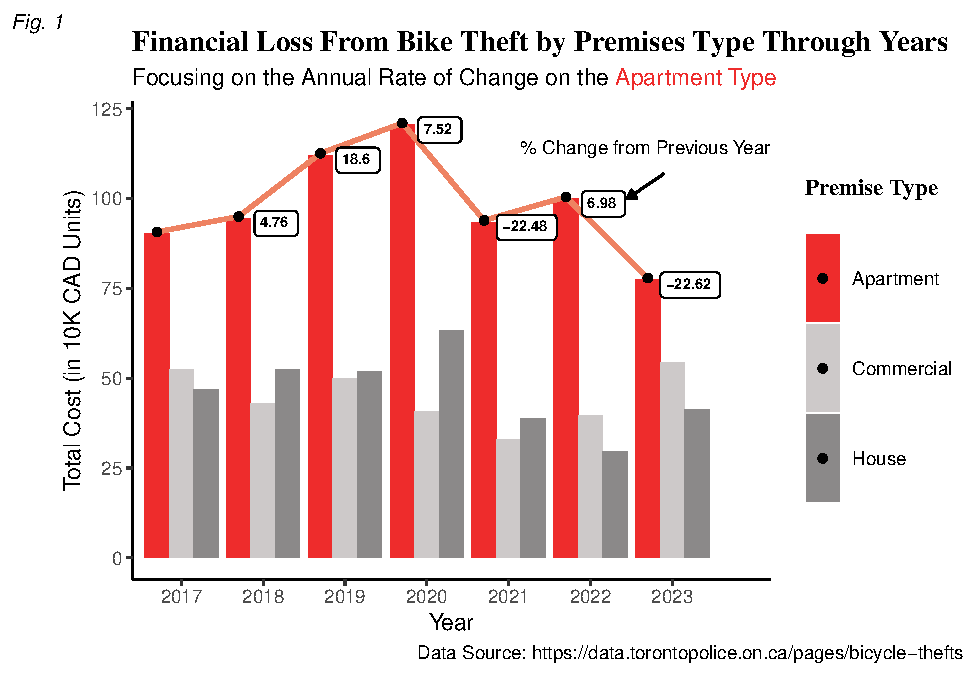
\includegraphics{Bike_Theft_files/figure-latex/unnamed-chunk-5-1} \end{center}

\newpage

\textit{\textbf{{When Are Your Bikes Most at Risk?}}}

\textbf{\footnotesize{Including Seasonal Trends and Daily Comparisons of Apartment Bike Theft Incidents}}

\indent Exploring bike theft patterns in the top three non-outdoor
locations, particularly in apartment settings, underscores the need to
investigate intricate temporal trends not obvious from year-over-year
comparisons. Analyzing time-specific data---covering both daily and
seasonal variations---helps pinpoint peak theft times, facilitating
precise intervention by bike owners and external agencies alike. This
approach recognizes the significant impact of human behavioural
patterns, which fluctuate widely over different times of the day and
seasons, on the susceptibility of bikes to theft, which introduces us to
the second graph.

\begin{center}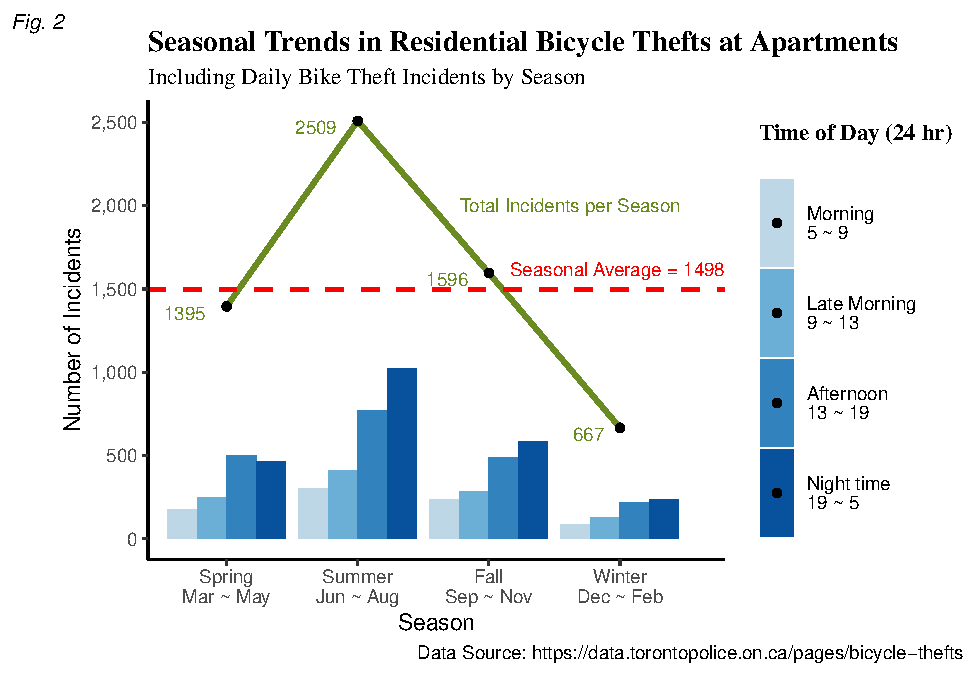
\includegraphics{Bike_Theft_files/figure-latex/unnamed-chunk-6-1} \end{center}

\indent Figure 2 presents a bar chart with dual dimensions: seasonal
variation and time of day, across four seasons, further divided into
four daily periods. The chart categorizes the four seasons, each
subdivided into four daily intervals of bike theft incidents along the
x-axis. This very grouping of time and deliberate visual arrangement are
designed to reveal the intricacies of temporal patterns while preserving
an overarching temporal view, with additional employment of colour
intensity on the bar to encode the time of the day, with darker tones
for later hours, enhancing the chart's clarity on when thefts occur.
This approach effectively reveals a trend of increasing bike theft from
morning to night, peaking at night. This suggests bikes left unsecured
overnight are at the highest risk, possibly due to lower pedestrian
traffic and reduced visibility. Afternoon incidents may occur as bikes
are left unattended when residents are away for work, whereas morning
incidents coincide with heightened bike use, reducing theft
opportunities. In addition, the line graph set at the top highlights
seasonal theft trends, showing a summer peak with 2,509 reported thefts,
well above the seasonal average of 1,498 incidents. Autumn sees a slight
decrease to 1,596 incidents, but is still above average, while spring
and winter fall below, with winter at 667 incidents---the lowest. The
contrast between summer and winter suggests warmer weather increases
bike usage and exposure to theft, whereas colder weather likely leads to
more bikes being secured indoors, reducing theft risks. Upon closer
inspection of the temporal categorization, the visual analysis
methodically segments bike theft incidents at apartments by season and
daily intervals, yet the division into daily intervals---while
reflective of typical daily activities---may not uniformly represent the
data, potentially masking subtler trends within each period. This could
be remedied by a finer temporal resolution that could provide a more
precise identification of peak theft times.

\textit{\textbf{{Which Stolen Bikes Find Their Way Home? }}}

\textbf{\footnotesize{Bicycle Recovery Rates Across Varied Types and Colors at the Apartment Area}}

\indent Indeed, the analysis of temporal factors underscores the
critical need for cyclists, particularly those living in apartments, to
exercise increased vigilance and implement strong bike security
measures, especially during nighttime and the summer months. This
emphasis on time and setting naturally extends the inquiry to the
characteristics of the bikes themselves and their influence on recovery
rates. Understanding which features of a bike correlate with higher or
lower recovery rates can provide essential insights for owners on
enhancing security measures or modifying bike features to make them less
appealing to thieves or easier to recover. Motivated by this, an
investigation into the residential bicycle recovery rates by type and
colour was undertaken.

\begin{center}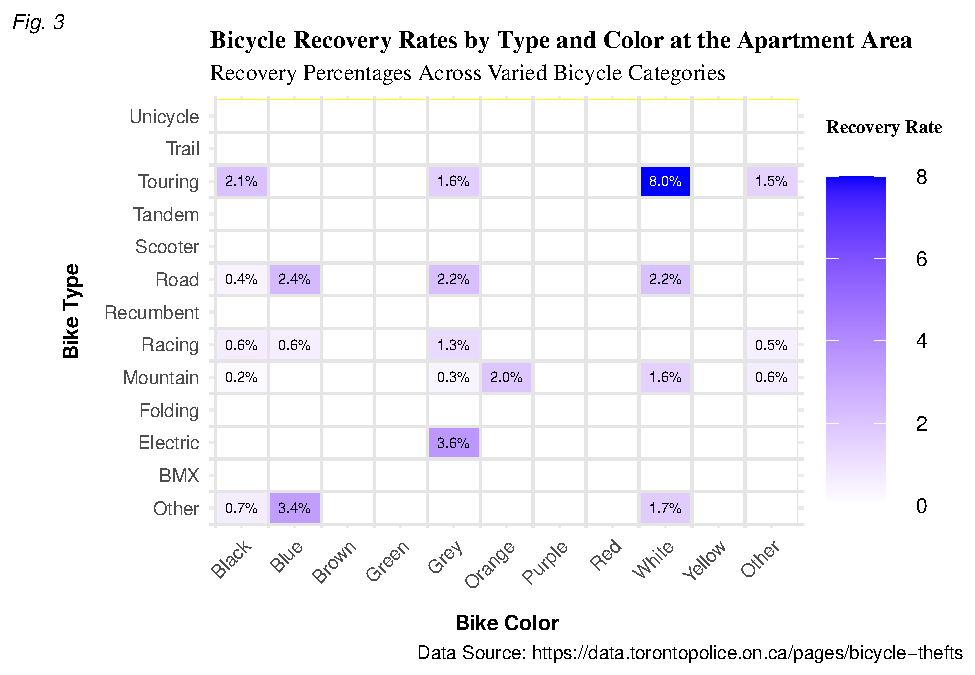
\includegraphics{Bike_Theft_files/figure-latex/unnamed-chunk-7-1} \end{center}

\indent Figure three's heatmap, which delineates bicycle recovery rates
by type and color, reveals that recovery percentages vary significantly
across different bike categories. This disparity is most pronounced in
the 8\% recovery rate for white touring bikes, markedly surpassing other
combinations of bike type and colour. This outlier suggests that white
touring bikes possess unique attributes conducive to their recovery,
such as high visibility, distinctive features, or robust community
support for reporting thefts and facilitating recovery. However, the
hypothesis that colour directly contributes to recovery success faces
challenges, notably the absence of recoveries for red or yellow
bikes---colours traditionally considered highly visible and thus
presumed to draw more attention from thieves. The data showcases
distinct variations in recovery rates among bike types, with touring,
road, and electric bikes exhibiting higher rates for specific colours.
This pattern suggests that the likelihood of recovery is influenced by a
bike's type and, to a more uncertain extent, its colour, given the noted
contradictions regarding colour visibility. Despite these insights, it's
crucial to acknowledge that even the highest recovery rates do not
exceed 10\%, with the second highest falling below 4\%. This reality,
coupled with the fact that most combinations of bike type and colour
result in non-recovery, highlights a sobering truth: the overwhelming
majority of stolen bikes are never recovered. Indeed, a closer
examination reveals a significant limitation: the oversimplification of
colour categories, which may obscure the true granularity of bike
colours and lead to potential miscategorization, skewing the analysis.
This aggregation could also explain the unexpected absence of recoveries
for typically high-visibility colours like red and yellow, questioning
the presumed influence of colour on recovery rates. Therefore, a remedy
would be to adopt a more granular colour classification system,
enhancing the precision of the analysis and potentially clarifying the
role of colour visibility in bike theft recoveries.

\textit{\textbf{{How Fast Should You Report?}}}

\textbf{\footnotesize{
Report Durations (log scale) by Bike Cost and Recovery Status (Missing vs. Recovered)}}

\indent The analysis brings to light two notable findings: the high
recovery rates for white touring and grey electric bikes. The
inconsistent patterns associated with colour suggest a more fruitful
investigation of bike types, the potential influence of price,
especially considering that
\href{https://tomsbiketrip.com/which-touring-bike-should-i-buy/}{touring}
and \href{https://gitnux.org/ebike-statistics/}{electric} bikes
typically reside in a higher price bracket compared to other types.
Price reflects not just the market value but also the design
sophistication of a bike, factors that extend beyond simple colour and
type considerations and may affect a bike's allure to thieves. However,
considering the limited success in recovery observed in previous
analyses, it becomes pertinent to investigate the efficacy of reporting
thefts to the police and the optimal timing for such reports in
enhancing the chances of recovery, to rebuild the confidence of bike
owners when facing stolen situations. Thus, exploring the interplay
between a bike's price, the timing of theft reporting, and the recovery
outcomes for these more expensive bike types offers a compelling next
step in our research.

\begin{center}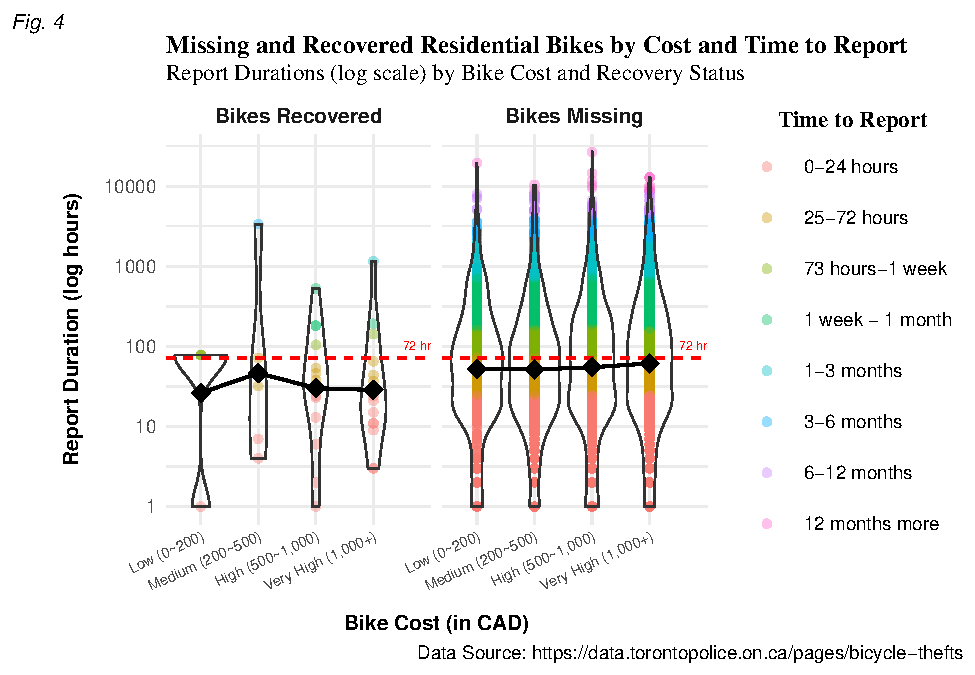
\includegraphics{Bike_Theft_files/figure-latex/unnamed-chunk-8-1} \end{center}

\indent Figure four presents a violin plot with a scatter plot overlay,
reinforcing the observation from previous graphs that most bikes remain
missing after being reported. The logarithmic scale on the y-axis
captures a wide range of reporting times, from immediate to
significantly delayed reports post-theft. A notable feature is the
72-hour benchmark, underscoring a critical window for timely reporting,
which is essential for recovery. The recovered bikes tend to cluster at
the lower end of the report duration scale, indicating that swift
reporting is a common factor in successful recovery cases, as
illustrated by the broader bases of the violins in these categories.
Conversely, the violins for missing bikes demonstrate a dispersed
distribution across the report duration scale, suggesting a more erratic
reporting timeframe. Interestingly, there is a subtle upward trend in
the average report time for unrecovered bikes as the cost increases,
defying expectations that higher-value bikes would be reported stolen
more quickly. This counterintuitive trend might stem from various
factors, including the need for owners to compile comprehensive
documentation for high-value bikes, which could delay the reporting
process. Indeed, this very analysis might not fully capture the
individual and situational factors affecting theft report timings,
particularly for high-value bikes, which are reported missing later than
expected. To mitigate this, integrating qualitative data through owner
surveys or interviews could reveal underlying causes for these reporting
delays.

\indent The last visual analysis suggests that despite a limited sample
size for recovered bikes, the data yields a valuable insight: promptly
reporting a bike as missing significantly enhances the probability of
recovery, regardless of the bike's value. Although the likelihood of
recovery is limited as suggested by previous analysis, the data
indicates that the opportunity for successful retrieval does indeed
exist.

\newpage

\textbf{\emph{Conclusion}}

\indent In conclusion, navigating bike safety in Toronto is a journey of
awareness and action. The data we have explored offers crucial insights
for cyclists in Toronto, illuminating the risks and offering strategies
to safeguard their cherished rides. Our analysis has shed light not only
on the seasonal and daily peak times for theft but also on the urgency
for timely theft reporting and heightened protection, particularly for
apartment dwellers. With this valuable knowledge in hand, cyclists can
navigate with increased confidence, take proactive measures during
high-risk periods, and advocate for improved security in vulnerable
areas. Together, we can foster a safer cycling environment and a
stronger, more vigilant community in Toronto.

\end{document}
